%&pdflatex

%\documentclass[preprint,10pt]{elsarticle}
\documentclass[10pt]{article}
\usepackage{fullpage}
\usepackage{hyperref}
\let\proof\relax
\let\endproof\relax
\usepackage{amsmath,amssymb,amsfonts,mathrsfs,amsthm}
\usepackage[titletoc,toc,title]{appendix}

%\usepackage{lineno}
\usepackage{array}
\usepackage[utf8]{inputenc}
\usepackage{listings}
\usepackage{mathtools}
\usepackage{pdfpages}
\usepackage[textsize=footnotesize,color=green]{todonotes}
\usepackage{bm}
%\usepackage{tikz}
\usepackage[normalem]{ulem}
\usepackage{hhline}
\usepackage{csquotes}
\usepackage{algorithm}
\usepackage[noend]{algpseudocode}
\usepackage{algorithmicx}

\usepackage{graphicx}
%\usepackage{subfigure}
\usepackage{subfig}

\usepackage{color}
\definecolor{forestgreen}{rgb}{0, 0.5, 0}

\renewcommand{\topfraction}{0.85}
\renewcommand{\textfraction}{0.1}
\renewcommand{\floatpagefraction}{0.75}

\newcommand{\vect}[1]{\ensuremath\boldsymbol{#1}}
\newcommand{\tensor}[1]{\underline{\bm{#1}}}
\newcommand{\del}{\triangle}
\newcommand{\curl}{\grad \times}
\renewcommand{\div}{\grad \cdot}
\newcommand{\td}[2]{\frac{{\rm d}#1}{{\rm d}#2}}
\newcommand{\pd}[2]{\frac{\partial#1}{\partial#2}}
\newcommand{\pdd}[2]{\frac{\partial^2#1}{\partial#2^2}}

\newcommand{\bs}[1]{\boldsymbol{#1}}

\newcommand{\equaldef}{\stackrel{\mathrm{def}}{=}}

\newcommand{\tablab}[1]{\label{tab:#1}}
\newcommand{\tabref}[1]{Table~\ref{tab:#1}}

\newcommand{\theolab}[1]{\label{theo:#1}}
\newcommand{\theoref}[1]{\ref{theo:#1}}
\newcommand{\eqnlab}[1]{\label{eq:#1}}
\newcommand{\eqnref}[1]{\eqref{eq:#1}}
\newcommand{\seclab}[1]{\label{sec:#1}}
\newcommand{\secref}[1]{\ref{sec:#1}}
\newcommand{\lemlab}[1]{\label{lem:#1}}
\newcommand{\lemref}[1]{\ref{lem:#1}}

\newcommand{\mb}[1]{\mathbf{#1}}
\newcommand{\mbb}[1]{\mathbb{#1}}
\newcommand{\mc}[1]{\mathcal{#1}}
\newcommand{\nor}[1]{\left\| #1 \right\|}
\newcommand{\snor}[1]{\left| #1 \right|}
\newcommand{\LRp}[1]{\left( #1 \right)}
\newcommand{\LRs}[1]{\left[ #1 \right]}
\newcommand{\LRa}[1]{\left\langle #1 \right\rangle}
\newcommand{\LRb}[1]{\left| #1 \right|}
\newcommand{\LRc}[1]{\left\{ #1 \right\}}

\newcommand{\Grad} {\ensuremath{\nabla}}
\newcommand{\Div} {\ensuremath{\nabla\cdot}}
\newcommand{\Nel} {\ensuremath{{N^\text{el}}}}
\newcommand{\jump}[1] {\ensuremath{\LRs{\![#1]\!}}}
\newcommand{\avg}[1] {\ensuremath{\LRc{\!\{#1\}\!}}}
\newcommand{\uh}{\widehat{u}}
\newcommand{\Bh}{\widehat{B}}
\newcommand{\fnh}{\widehat{f}_n}
\renewcommand{\L}{L^2\LRp{\Omega}}
\newcommand{\pO}{\partial\Omega}
\newcommand{\Gh}{\Gamma_h}
\newcommand{\Gm}{\Gamma_{-}}
\newcommand{\Gp}{\Gamma_{+}}
\newcommand{\Go}{\Gamma_0}
\newcommand{\Oh}{\Omega_h}

\newtheorem{theorem}{Theorem}[section]
\newtheorem{lemma}[theorem]{Lemma}
\newtheorem{proposition}[theorem]{Proposition}
\newtheorem{corollary}[theorem]{Corollary}

\newenvironment{definition}[1][Definition]{\begin{trivlist}
\item[\hskip \labelsep {\bfseries #1}]}{\end{trivlist}}
\newenvironment{example}[1][Example]{\begin{trivlist}
\item[\hskip \labelsep {\bfseries #1}]}{\end{trivlist}}

\newcommand{\eval}[2][\right]{\relax
  \ifx#1\right\relax \left.\fi#2#1\rvert}

\def\etal{{\it et al.~}}


\def\arr#1#2#3#4{\left[
\begin{array}{cc}
#1 & #2\\
#3 & #4\\
\end{array}
\right]}
\def\vectwo#1#2{\left[
\begin{array}{c}
#1\\
#2\\
\end{array}
\right]}
\def\vecthree#1#2#3{\left[
\begin{array}{c}
#1\\
#2\\
#3\\
\end{array}
\right]}
\def\vectfour#1#2#3#4{\left[
\begin{array}{c}
#1\\
#2\\
#3\\
#4\\
\end{array}
\right]}

\newcommand{\G} {\Gamma}
\newcommand{\Gin} {\Gamma_{in}}
\newcommand{\Gout} {\Gamma_{out}}

\newcommand{\note}[1]{{\color{violet}#1}}
\newcommand{\reviewerOne}[1]{{\color{blue}#1}}
\newcommand{\reviewerTwo}[1]{{\color{red}#1}}
%\newcommand{\remark}[1]{\textbf{\color{red}#1}}

\newcommand{\tri}{{\rm tri}}
\newcommand{\sqr}{{\rm quad}}

\newcommand{\refhex}{\widehat{\mathcal{H}}}
\newcommand{\reftet}{\widehat{\mathcal{T}}}
\newcommand{\refwedg}{\widehat{\mathcal{W}}}

\newcommand{\refpyr}{\widehat{\mathcal{P}}}
\newcommand{\refpyrf}{\widehat{\mathcal{P}}^f}
\newcommand{\refpyrfq}{\widehat{\mathcal{P}}^{\sqr}}
\newcommand{\refpyrft}{\widehat{\mathcal{P}}^{\tri}}


\newcommand{\hex}{{\mathcal{H}}}
\newcommand{\tet}{{\mathcal{T}}}
\newcommand{\wedg}{{\mathcal{W}}}

\newcommand{\pyr}{{\mathcal{P}}}
\newcommand{\pyrf}{{\mathcal{P}}^f}
\newcommand{\pyrfq}{{\mathcal{P}}^{\sqr}}
\newcommand{\pyrft}{{\mathcal{P}}^{\tri}}

\newcommand{\half}{1/2}

\newcolumntype{C}[1]{>{\centering\let\newline\\\arraybackslash\hspace{0pt}}m{#1}}

%% d in integrand
\newcommand*\diff[1]{\mathop{}\!{\mathrm{d}#1}}

\makeatletter
\renewcommand\d[1]{\mspace{6mu}\mathrm{d}#1\@ifnextchar\d{\mspace{-3mu}}{}}
\makeatother

\newcommand{\squareface}{[-1,1]^2}

%\journal{Journal of Computational Physics (JCP)}

\date{}
\author{Jesse Chan, John A.\ Evans}
\title{Response to reviewers: ``Multi-patch discontinuous Galerkin spline finite element methods for time-domain wave propagation''}

\graphicspath{{./figs/}}

\begin{document}

\maketitle

\note{We thank the two anonymous reviewers for their feedback.  We describe steps taken to address reviewer comments and suggestions, which are described in the following response.  Revisions in the manuscript are also colored \reviewerOne{for Reviewer 1} and \reviewerTwo{for Reviewer 2} for ease of identification.  We have modified the title to ``Multi-patch discontinuous Galerkin isogeometric analysis for wave propagation: explicit time-stepping and efficient mass matrix inversion'' in order to provide more description of the material in the paper.  We have also made minor changes in nomenclature, referring to micro-elements simply as ``elements'' and referring to subdomains $D^k$ as ``patches'' and correcting an inconsistent definition of the trace and inverse inequality constants.  A figure has been added to further clarify these notational changes.  These changes are also highlighted in {\color{forestgreen} green} in the revised manuscript.   We hope these revisions improve the readability of this paper and its suitability for the audience of CMAME.}  

\section{Reviewer 1}

The paper describes a new approach to handling the patch dependent mass matrix in for spline based finite element methods in order to improve computational efficiency. The author also introduce a novel approach to determining improved knot locations for B-splines. Finally the authors explore the time step restriction for B-spline methods.

I believe the work is worthy of publication once the comments below (particularly those concerning the time step restriction) are resolved.

\begin{enumerate}
\item One thing that I got a bit turned around in the paper is the meaning of $h$ throughout the text. *I think* that in some places, $h$ is the 'micro-element' size and in other places it is the 'patch size'; sometimes the patch size is denoted $H$ as well. This was particularly confusing when talking about time step restrictions, since on page 13 $h$ means patch size and the micro-element size shows up $C_{I}$ and $C_{T}$. Similarly, the $h$ which shows up in the introduction when talking about time step size (page 2) is the patch size when talking about the finite element methods (since patch size is element size in the this case) but micro-element size when talking about spline methods (*I think*).

\note{We have modified the revision in a number of ways to address this comment.  First of all, we have removed all mention of ``micro-element'' and instead refer only to ``patches'' and ``elements'' (which previously were referred to as micro-elements).  This is consistent with the standard terminology in the isogeometric analysis community.  Second, we have modified the revision to ensure that $H$ always refers to the patch size and $h$ refers to the element size.  Third, we have included a figure to clearly demonstrate what $H$ and $h$ are in a visual manner.  Fourth, we have included a remark noting that $H = h$ for a $C^0$-continuous or discontinuous finite element method, and hence the terms patch and element are interchangeable for this setting.  We hope these modification clarify the manuscript.  }

\item I'm not completely convinced that the time step for the B-spline methods is that much better than for polynomials. If we use a B-spline approximation that if $p$-th order accurate with $K$ micro-elements, this results in roughly $K$ degrees of freedom. Assume that the domain is of length $H$, this results in a time step that if proportional to $H / K p$. Now, presumably to get a finite element solution of roughly the same order of accuracy, I need roughly the same number of degrees of freedom. To do this, we would need our finite element mesh to have $E = K / p$ elements (so that the total degrees of freedom is roughly $E p = K$).  Each of these element is of size $H / E = p H / K$, and thus the time step restriction if $(H / E) / p^2 = H / K p$ which is the same as for the B-spline method. This back of the envelop calculation suggests that they have roughly the same time step restriction, but does not consider the scaling constant that comes into both of these. I think that by dividing by $K$ in the Figures 7 and 8 there is a factor of $p$ that is being lost since $K$ scales with $p$. (For splines $H / K$ is similar to $h / p$ polynomials, since both are approximately an average node spacing.)

\note{We thank the reviewer for their comments.  We believe the discrepancy lies is in the statement ``presumably to get a finite element solution of roughly the same order of accuracy, I need roughly the same number of degrees of freedom''.  Numerical experiments in the spline literature show that instead, for a fixed order $p$ and similar mesh size $h$, splines are more efficient per degree of freedom than $C^0$ finite elements \cite{evans2009n} (with the caveat that those degrees of freedom are more tightly coupled).  
\\
\\
Thus, assuming a physical patch (element) of size $O(1)$, a degree $p$ polynomial method would have a timestep restriction of $O(1/p^2)$.  A spline method would have a timestep restriction of $O(1/(pK))$, and with $K = O(p)$, this results in the reviewer's observation that a spline method would have an $O(1/p^2)$ timestep restriction as well.  However, what this does not account for is the fact that the spline also increases the mesh resolution of by a factor of $O(1/K) = O(1/p)$.  Thus, to achieve the same resolution as a spline space of degree $p$ and $K$ elements, a polynomial finite element method would require a mesh of size $O(1/p)$, which would decrease the timestep restriction to $O(h/p^2) = O(1/p^3)$.  Thus, splines allow for a factor of $O(p)$ increase in the time-step over a $C^0$ finite element method of equivalent $h$ and $p$ resolution.  
\\
\\
We have added a section explaining this in the revised manuscript.
}

\item In section 3 (definition of B-spline basis) it could be helpful to readers who have minimal exposure to B-splines to add a few more broad details. In particular, I think that it would be useful to write down the final approximation once the degrees of freedom have been set and point out/remind the reader B-splines is not an interpolant of the function values at the knots (i.e., the approximation does not pass through the degrees of freedom and hence there is no problem with having multiple values at the same physical point).

\note{We have added a brief discussion of B-spline coefficients to the revised manuscript, and have noted that they should not be treated as interpolatory basis functions.}

\item I was a little confused by the iterative smoothing procedure outlined on page 8 for the knot locations. In particular, when (2) is used what exactly are the $\hat{n}_{i}$ values. At first I thought that $\hat{x}_{i} = \frac{2}{K}(i-1)-1$ (i.e., equally spaced between $[-1,1]$), but then footnote 3 seems to contradict this, since the $\tau_{i}$ cannot be equally spaced.

\note{We apologize; there is an error in (2), and the $\hat{x}_i$ should be $\hat{x}_j$.  We have corrected this in the revised manuscript.
\\
\\
The $\hat{x}_i$ points are in fact equally spaced points on $[-1,1]$.  We have noted in the revision that (2) can be interpreted as an attempt to reverse-engineer a knot vector which produces equispaced Greville abscissae. The goal is to produce new knot locations $\tilde{\xi}_i$ for which the Greville abscissae are less clustered towards the endpoints.  
}

\item Specific Comments:
\begin{enumerate}
\item [page 2, lines 20-29] As hinted to above, I think that you should spell out what $h$ is in each of the cases in this paragraph (since I think that the mean different things).

\note{We agree, and have added descriptions of both patch size $H$ and mesh size $h$ to this paragraph.}

\item [page 3, line 6] Not necessary, but you may want to mention what $\phi$ is.

\note{We have specified that it represents some concentration.}

\item [page 3, line 14] You may want to mention this assumes that $c$ is a constant wave speed as well as define $p$ and $\vec{u}$ (and state the dimension of $\vec{u}$)

\note{We have added a description of $p$ and $\bm{u}$.  However, to the authors' understanding, $c$ does not necessarily need to be constant for this formulation to be applicable (see, for example \cite{chan2017weight1,mercerat2015nodal}). }

\item [page 3, line 26] This equations should still include $c$ I believe, and you may want to state that the $f$ here and the $f$ above are different.

\note{We thank the reviewer for their careful reading; we have corrected this in the revision.}

\item [page 3, line 33] Is it true that NURBS is always used, or is it just often used? (I don't know for certain)

\note{We thank the reviewer for their question.  For spline discretizations, NURBS are the most commonly used type of geometric mapping.  Additionally, NURBS mappings also include isoparametric mappings.  We have removed the NURBS reference in the revision, since the method can be used for more general geometric mappings as well.}

\item [page 4, line 42] Might be worth stating that energy stable in this case is that $d/dt\sum_{k}(v, v) \le 0$.

\note{We have added this to the revision.}

\item [page 7, line 45] It is hard to see in the figure that the points are clustering. Not sure how this could be improved, perhaps plotting the optimal points all on the same graph?

\note{We note that ``clustering'' may not be an appropriate description of the point behavior, and have modified this in the revision to read: ``the gap between each of the boundary knots and the closest interior knot grows'' as $r$ increases.}

\item [Page 8, line 9] should $j$ run from $1$ to $K$?

\note{We believe $j$ should run to $p+K$, which is the total number of degree $p$ B-spline basis functions for a knot vector containing $K$ elements.}

\item [page 12, line 48] reference 11 describes the Galerkin difference methods in 1-D, and does not consider mapped domains. Perhaps the reference should be moved a few words earlier?  

\note{We have removed this reference, as the cited work references a paper in progress.}

\item [page 13, lines 23, 28, 40] Should there be absolute values around the eigenvalues ($A_{h}$ have non-positive real components) for stability.  [page 13, line 34] Perhaps the sentence on line 44 "For illustation..." should be moved up to before the advection example begins (line 34)?

\note{We thank the reviewer for their careful reading; this has been corrected in the revision.}

\item [page 13, line 37] Should $a_{\mbox{sym}}$ be included too?

\note{We specify $a_{\mbox{sym}}$ in terms of $a(u,v)$ in the previous few lines; we have only given an explicit expression for $a_{\mbox{skew}}$ since the complex conjugate is introduced (which was not present in the original form $a(u,v)$).}

\item [page 13, line 56] Perhaps $H$ should be used instead of $h$ so as not to be confused with previously defined $h = H / K$?  [page 14, line 13] Should the $\beta$ here be a $c^2$?  [page 14, line 13] Perhaps $C_{p}$ should be defined earlier, and used in the other expressions?

\note{Yes, and we thank the reviewer for pointing these issues out.  We have also modified the revision so that $C_p$ is introduced earlier, and have mentioned that the trace and inverse inequality constants depend on $h$.}

\item [page 14, line 13] Strictly speaking $\Delta t$ should also have a constant multiplying due to the stability region of the time stepping method.

\note{We have added a constant describing the impact of the stability region of the time-stepping method.}

\item [page 15, line 35] You may want to point out that the numerical stability issues are in the calculation of the points not the PDE approximation using the points.

\note{We thank the reviewer for their suggestion, and have clarified this in the revision.}

\item [page 15, line 53] I had to read the sentence "In contrast, not only..." several times due to all the negations. Perhaps this sentence could be reworeded.

\note{We have broken this sentence into two: ``In contrast, knot smoothing does not significantly decrease accuracy.  Additionally, the approximation power of spline spaces under knot smoothing is actually improved for certain functions''.  We hope this improves readability.}

\item [page 16, line 26, 35] In the table captions I think that a scaling by $K$ is missing.

\note{We thank the reviewer for their careful reading; this has been corrected in the revision.}

\item [page 17, line 47] Should you define how you are computing the approximation? I assume that you mean that you are doing an $L^2$ projection of the function to the spline representation (but this is never stated). You may also want to state how you are computing the $L^2$ error (presumable integration using high order quadrature?)

\note{We agree with the reviewer, and have clarified how the approximation is computed, including a description of the composite Gaussian quadrature rule used.}

\item [page 19, line 19] You may want to consider adding labels to the x-axis.

\note{We have added $x$-axis labels to the revision.}

\item [page 19, figs 10 and 11] Would it be useful showing both Figures 10 and 11 with the same $p$ and $K$ and using the same x-axis (one use $k$ and the other $k / dof$) so that the effects of the approximation can be compared between the two?

\note{We have modified both figures to have the same axes.  Additionally, in order to facilitate a comparison between the two, we have switched to approximating the same function in both Figures 10 and 11.  }

%\item [page 19, line 52] As above you may want to explicit about how you are approximating the function in the approximation space.

\item [page 19, line 53] Should the word "elements", really be "micro-elements"?  (same in caption of Fig. 13). You may also want to make clear that you are using a single polynomial "element" not a mesh of elements (at least this is what I gather you are doing).

\note{As previously mentioned, we have replaced the term ``micro-element'' with ``element'' throughout the paper, so this comment is no longer applicable.}

\item [page 20, line 57] Might be better to say "are closer than in the one-dimensional case" (I found the wording confusing since you are not comparing the one-dimensional and two-dimensional cases, but the two knot distributions in each case).

\note{We agree, and have corrected this issue in the revision.}

\item [page 20, line 58] I had to reread the sentence ``This suggests...'' several times to understand what was being said. My understanding of the logic is that since the errors are same AND the timestep for the smooth knots is larger, a larger timestep can be taken to get the same spatial error. And that this is not true in the one-dimensional case because you would need to increase the number of knots for the smoothed distribution to get the same error and thus needed a smaller timestep.  

\note{We apologize for the confusion, and have restructured this sentence in the revision: ``This suggests that the use of smoothed knots instead of uniform knots can improve solver efficiency, since it is possible to take a larger maximum stable timestep without reducing accuracy.  A more rigorous study of this claim is still required.''  Additionally, we have clarified that the improvement in efficiency is not due to the dimension of the problem, but the presence of a curvilinear warping (which does not naturally appear in 1D problems).}

\item [page 21, fig 14] The placement of the $10^4$ in the figures looks like its in the axis label, but I think that it is really scaling the axis.  [page 21, line 40] You may want to put the $\alpha$ factor in the caption so it is more self contained.

\note{We thank the reviewer for their suggestions.  We have addressed both of these points in the revision by switching to a log-log axis and modifying the caption to include $\alpha$.}

\item [page 22, sec 5.4.1] It should be pointed out somewhere in this section that you are considering a 1-D problem. Also, is it worth showing the spectrum in any of these cases? Wondering since RK stability regions are not circles, but a peanut-shaped region so spectral radius is not the full story for a stable time step.  

\note{We agree, and have added plots of the spectra for the advection equation.  These plots further and illustrate how the spectra depends on both the penalty parameter $\tau$ and the knot distribution.}
%\textcolor{red}{TODO}

\item [page 23, line 48] Does this suggest that upwind fluxes should be used instead of the penalty flux? Is similar behavior seen for the wave equation?

\note{For the constant coefficient advection equation, the penalty and upwind fluxes coincide, so we cannot draw a conclusion on the use of penalty or upwind fluxes from this specific experiment.  Additionally, it is unclear whether this phenomena holds for more complex scenarios where the upwind and penalty fluxes differ (for example, curvilinear meshes or discontinuous wave speeds).  
\\
\\
Similar behavior is observed for the wave equation, and we have mentioned this in the revised manuscript.}

\item [page 24, Fig 18c,d] What is the black line in these figures? What is $h^{11}$ and what does it represent?  

\note{We have clarified in the caption that the black line represents the exact dispersion relation in Figure 18c, while in Figure 19c, the black dotted line is the slope $h^{11}$, which corresponds to the theoretical rate of convergence of the dispersion error for $p=4$.}

\item [page 24, line 43] From the figure, it seems that changing $K$ does more than just shifting things by a constant.

\note{We have clarified this in the revision to specify that $h$-refinement shifts the dispersion error curve by a constant number of wavelengths per degree of freedom. }

\item [page 24, line 50] How does $\tau$ effect the dispersion error results?

\note{As $\tau\rightarrow 0$, we observe that the dispersion error increases for a larger number of wavelengths per degree of freedom.  We have included plots for reference here.  In the revision, we have added a discussion of this in a footnote.}
\begin{figure}
\centering
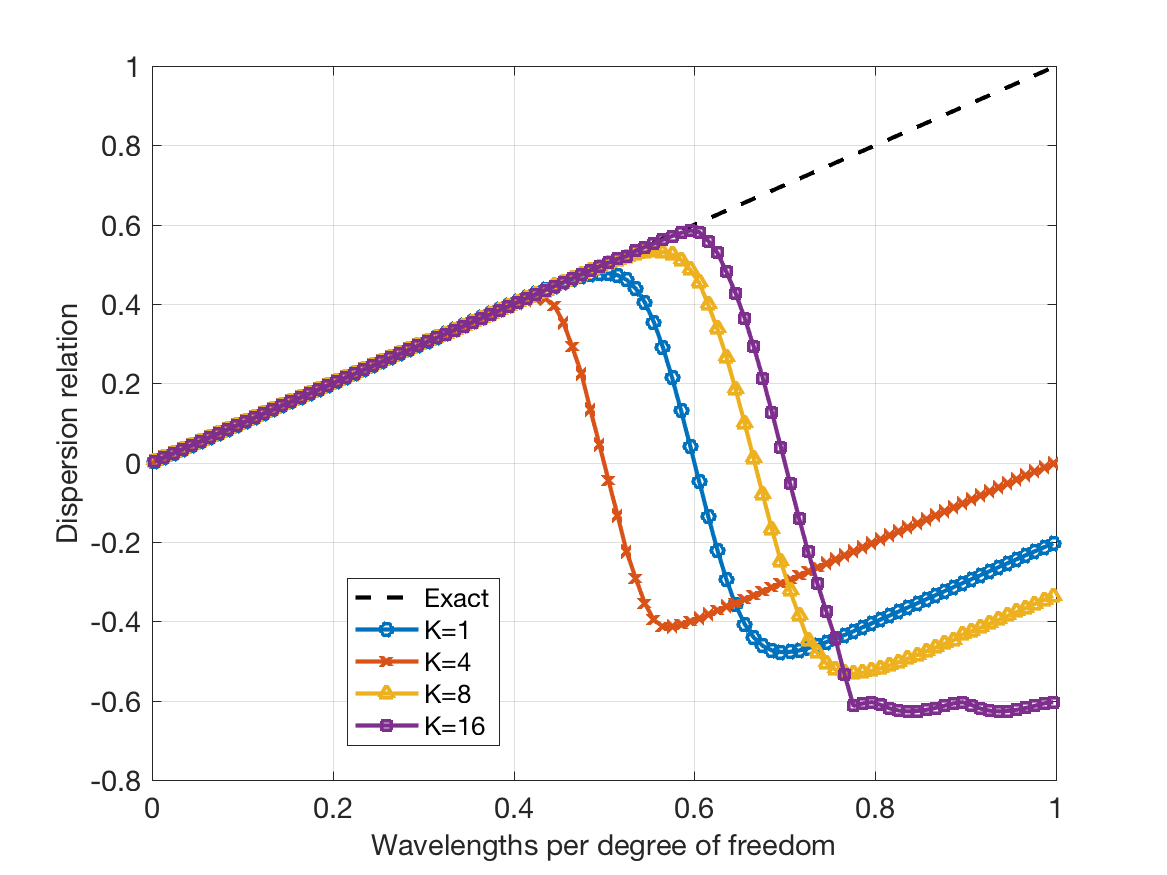
\includegraphics[width=.4\textwidth]{tau0dispersionRelation.png}
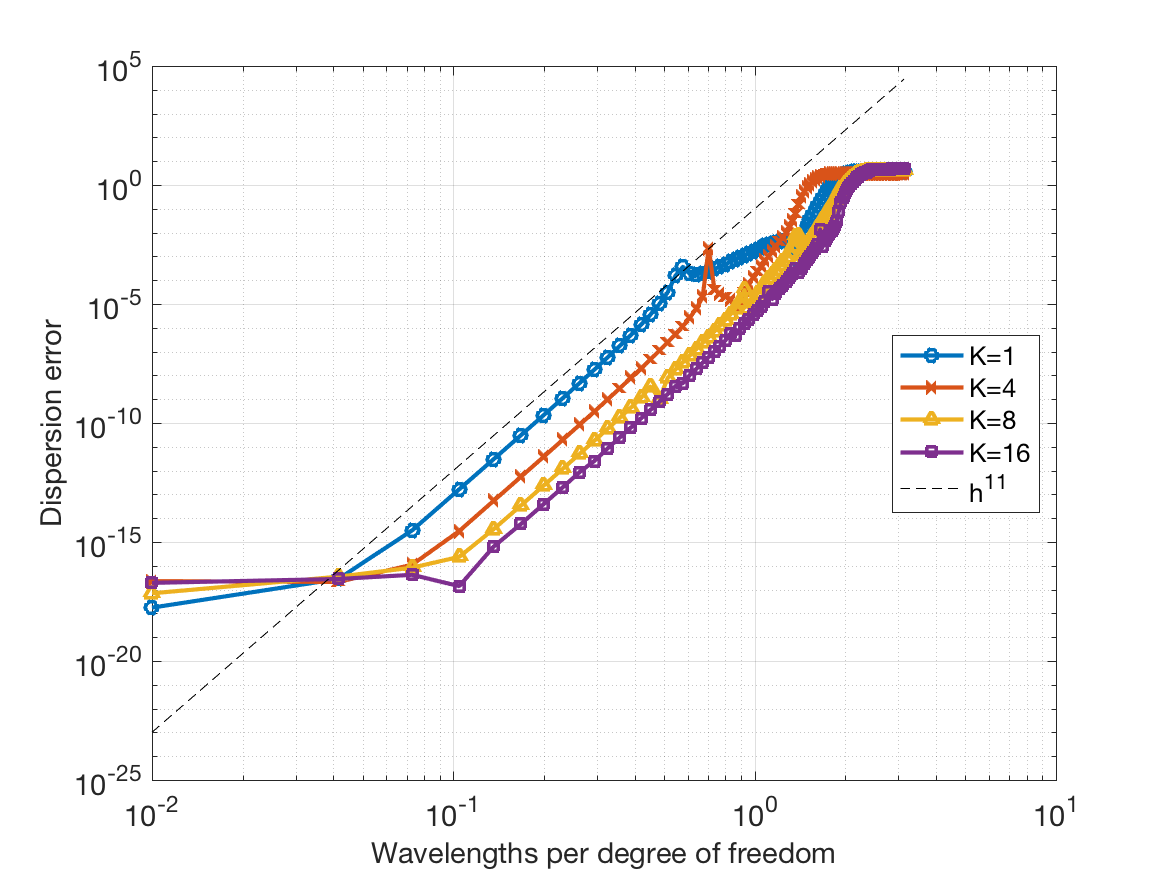
\includegraphics[width=.4\textwidth]{tau0dispersionError.png}
\caption{Dispersion relation and dispersion errors for $p=4$ and $\tau = 0$.  }
\end{figure}

\item [page 24, sec 5.5] Are the eigenvalues just sorted to determine which discrete eigenvalues correspond to the exact eigenvalues? Would this explain the ``blip'' in the error for the uniform mesh? Also, how are the eigenvectors normalized in computing the error?  

\note{Yes, the eigenvalues are sorted by magnitude.  The eigenvectors are sorted by the magnitude of the corresponding eigenvalue, and the normalization constant for a discrete eigenvector is computed by projecting the exact eigenvector onto the span of that single discrete eigenvector.  
\\
\\
The ``blip'' in the error corresponds to a very fortuitous aliasing error for $p=4$, where the discrete eigenvector on the uniform mesh matches the exact eigenvector almost exactly due to the matching of the uniformly spaced knot locations with zeros of the exact eigenvector.  It does not appear for smoothed knots since the knot locations are no longer uniformly spaced. }

\end{enumerate}
\end{enumerate}


\section{Reviewer 2}

This work presents efficient explicit time integration techniques in the context of isogeometric analysis applied to wave propagation problems. The method couples B-spline patches weakly by means of standard Discontinuous Galerkin techniques. The consistent mass matrix is block-diagonal and can be inverted patch by patch separately. The main contribution of the paper is an efficient strategy to invert the mass matrix in the context of curved geometries. The approach utilizes the tensor structure of the B-spline spaces and maintains higher order accuracy, which is critical. A secondary contribution is a study, based on the theory of n-widths, in which the spline knot vector is optimized to obtain optimality in the $L^2$-norm. It is shown that the spline spaces based on such a knot vector have slightly improved approximation properties of the medium to high modes in the spectrum, although the approximation of the low modes is slightly decreased. The improved approximation
properties of the high modes additionally lead to improved critical time step size. It is furthermore shown that the weak treatment of patch continuity can have a positive effect on the critical time step.

The paper is well written and is tackling an important topic in finite element analysis. I approve the manuscript for publication if some of the following matters are taken into consideration.

\begin{enumerate}
\item The main contribution, which is the efficient inversion of the mass matrix (approximately) is undersold, however. It would be good to show more numerical evidence, such as in Figure 12b, that shows that high order accuracy is maintained.

\note{We have added another 2D experiment comparing approximation errors, and have also added two numerical experiments comparing errors for the 2D wave equation using both the inversion of the curvilinear mass matrix and the inversion of the weight-adjusted approximation.} 

\item A lot of attention is spend on the improvement of the knot vector while little gain is achieved w.r.t accuracy or robustness. Perhaps the greatest efficiency here is w.r.t the gain in critical time step. The authors study the spectral radius and the constants in trace inequalities. Although this provides some evidence; why not directly estimate the critical time step by solving an eigenvalue problem and check if is tight. Then one can show using non-dimensional plots how the the critical time-step behaves.  

\note{We agree that the greatest efficiency gain here is likely with respect to the gain in critical time step.  For the advection equation and first-order wave equation, the maximum stable timestep size is directly tied to the spectral radius, with a constant of proportionality associated with the chosen explicit timestepper.  For the second-order wave equation, the maximum timestep size may indeed be attained from an eigenproblem, but we note that it may be equivalently attained from the square root of the spectral radius.  In this direction, we have added a paragraph to the paper noting the relationship between the maximum stable timestep and the spectral radius for the second-order wave equation.  We have further added plots of the square root of the spectral radius for the second-order wave equation to explicitly study the impact of polynomial degree $p$ on the maximum stable timestep size.}

\item Please introduce some equation numbering of the most important equations. Please proofread all equations again. I found several typo's but there may be more. Here is a list with more specific comments, fixes, etc.

\begin{enumerate}
\item Combined comments: [page 2, line 5]  geo-metrically i.s.o  ge-ometrically.  [page 2, line 12] requires the inversion of a 'sparse' matrix.  [page 3, line 25 and 26] The equation is different. There is a time derivative on the righthand side and a factor $(1/c^2)$ in front of the time term.  [page 3, line 50]                  denote the neighboring element 'sharing' a face.  [page 3, line 51] The jump 'and average' of .  [page 3, line 58] remove 'rule'

\note{These points have been corrected in the revision.}

\item page 3, line 45 -                [16,18]

\note{References [16, 18] refer to the inversion of a weighted mass matrix.  This line refers instead to constants in trace and inverse inequalities, which are first described in [14].  We have also added two additional references on explicit expressions for constants in trace and inverse inequalities to further clarify this.  }

\item page 4 and 5 -                  section 2.1 and 2.3 - complete the formulations. This is sloppy. 'Find ??.. such that for all??'

\note{The three formulations have been expanded as recommended in the revision.}

\item page 5                               define $x$ and $\hat{x}$

\note{The coordinates $x$ and $\hat{x}$ have been defined on page 3, line 35 of the original submission.}

\item page 5, line 6 -                  'pulled back' i.s.o 'mapped'

\note{We have added ``pulled back'' to clarify this sentence. }

\item page 5, line 14 -                where $G_{ij}$ is the inverse of the Jacobian matrix. 'a matrix of geometric change of variables' ?

\note{We have added the description of $G_{ij}$ as the inverse of the Jacobian matrix of the mapping, and have added two references showing that this matrix is also referred to as ``metric terms'' or ``geometric factors'' in the literature.}

\item page 6, line 47 -               [3, 12, 24] add the reference of the spline book by schumaker.

\note{We have added the reference to ``Spline functions: basic theory'' by Larry Schumaker.}

\item page 11, line 9-10             Remove the line "The extension of this work to NURBS approximations ??.". What you say in this sentence                                            is false. The mass matrix is not tensorizable in the case of NURBS. Obviously you can extend the approach given here, but in that case show how that is done.

\note{We have added a section describing how to generalize the weight-adjusted mass matrix inverse to rational NURBS basis functions.  }

\item page 11, line 40                Poor notation of this equation. Firstly, you have not defined multi-dimensional B-spline basis functions. Secondly, the pull back in combination with the same representation of the basis functions in physical and reference domain is poor notation.

\note{Multi-dimensional B-spline basis functions are defined in Section 3.3 of the original submitted manuscript.  We have moved this section such that it is now right after the section defining univariate B-spline basis functions.  We have also corrected the notation by introducing the inverse of the reference-to-physical geometric mapping.  }

\item page 12, line 33                Typo in equation. I think you mean ``$M_{1/J} = \ldots$'' i.s.o. ``$M^{-1}_{1/J} = \ldots$''.

\note{We thank the reviewer for their careful reading; this has been corrected in the revised manuscript.}

\item Combined comments: [page 12, line 40]                "The application of $M_{1/J}$ can be performed efficiently in a matrix free fashion". Just precompute it once and  use it repeatedly in the time integration algorithm.  [page 12, line 37]           You can write $\hat{M}$ using Cholesky as $L^T L$ and write $M^{-1} \approx L^{-T} W L^{-1}$ where $W = (L^{-1}  M_{1/J} L^{-T})$.   You can precompute $W$.

\note{We have added a note that one can also precompute and store this matrix.  However, $M_{1/J}$ does not admit a Kronecker product structure due to the $1/J$ weighting.  
%However, we note that this can increase storage costs and require more data movement, which can lead to slower runtimes on many-core architectures such as GPUs .  Additionally, the cost of the matrix-free application of $M_{1/J}$ can be combined with existing steps in explicit solvers to further reduce costs \cite{chan2016weight1}. 
This is not as problematic if only $M_{1/J}$ is stored, since it is sparse.  However, computing $W = (L^{-1}  M_{1/J} L^{-T})$ produces a three-dimensional dense matrix, and requires the same storage and computational work as explicitly pre-computing and storing the original weighted mass matrix. }

\item Combined comments: [page 12, line 57]     For reduced quadrature reference [Hiemstra, 2017, Schillinger, 2014].  [page 13, line 5]                 [37] is not a quadrature free method.  It proposes a different way of performing quadrature, which scales much better with regard to polynomial degree $p$.  

\note{We thank the reviewer for their comments, and have fixed both of these points in the revised manuscript.}

\item page 13, line 15                This sentence is not true. Although a Cholesky solve is not scalable, you have to perform $3n^2$ ($n$ is dim of 1D space) of them per patch since you are using the univariate operators. This is very scalable!  

\note{We thank the reviewer for pointing this out.  This is true; however, parallelizing over each of the $3n^2$ Cholesky solves also requires significantly more memory (due to the fact that the Cholesky backsolve requires storage of previous).  For accelerator and many-core architectures such as GPUs, this can lead to slower runtimes \cite{chan2017weight}.  We have added a footnote to the revised manuscript mentioning this.  }

\item page 13, line 31                Typo. $A_h - A_h^T$ i.s.o. $A_h - A_h$. Same typo as in line 32.

\note{We have corrected this in the revision.}

\item page 20, Figure 13           What does polynomial refer to here? Also, why not use a log-log scales for these plots (on x-axis use log of univariate number of dofs)

\note{We have specified that ``polynomial'' refers to a high order polynomial approximation.  We have also changed the semi-log scales to log-log scales in the revision.}

\item page 20, Figure 12b         This is a good Figure. I would show this for all the computations. For the 3D problem you could look at the relative difference in solution (in the $L^2$ norm) with respect to the consistent collocation mass.  

\note{We have added a few more experiments comparing approximation errors, and have added one plot comparing multi-patch DG errors using both the full weighted mass matrix inverse and the weight-adjusted approximate mass matrix inverse.  The high computational cost of computing fully dense inverses of 3D curvilinear mass matrices makes a detailed comparison in 3D infeasible.  Additionally, the comparison to collocation spline methods is outside of the scope of this work, and will be investigated in future work. }

\item Combined comments: [page 21, Figure 14]           Use a log-log scales for these plots (on $x$-axis use log of univariate number of dofs), [page 26, line 35]     integrate spline spaces to sufficient accuracy.  

\note{These have been corrected in the revision.}


\end{enumerate}
\end{enumerate}


\bibliographystyle{unsrt}
\bibliography{dgpenalty}

\end{document}